%!TEX root = ../../main.tex


A primeira fase do treinamento dos modelos foi conduzida utilizando a arquitetura LeNet. Nesta fase, foi realizada uma busca em \emph{grid} por todos os hiperparâmetros previamente definidos, conforme Seção \ref{sec:modelos}, e considerando as duas abordagens definidas conforme a Seção \ref{sec:preparacao}, gerando um total de $72$ modelos a serem treinados e testados. Para estes modelos, excluindo aqueles que se tornaram degenerados, utilizou-se a métrica \emph{F-Score} como referência para um melhor desempenho.

O melhor dos modelos baseados na arquitetura LeNet para cada uma das abordagens consideradas encontram-se dispostos na Tabela \ref{tab:lenet}, juntamente com os hiperparâmetros utilizados pelos mesmos.

\begin{table}[h]
\centering
\caption{Detalhamento dos melhores resultados obtidos com a arquitetura LeNet.}
\label{tab:lenet}
\resizebox{\textwidth}{!}{\begin{tabular}{ccccccc}
\toprule
\textbf{Abordagem} & \textbf{Otimizador} & \textbf{\emph{Patience}}  & \textbf{Função de Ativação} & \textbf{Acurácia} & \textbf{\emph{F-Score}} & \textbf{EER} \\
\midrule
Abordagem A & RMSprop & 5 & ReLU & $0.9865$ & $0.9755$ & \\
Abordagem B & Adam & 10 & ELU & $0.8361$ & $0.8159$ & $12.5245$ \\
\bottomrule
\end{tabular}}
\end{table}


Os gráficos da Figura \ref{fig:treinamento-lenet} denotam o histórico da perda (\emph{loss}) e acurácia para o conjunto de treinamento e validação destas redes. Nota-se que nenhuma delas chegou ao limite máximo de épocas possíveis, interrompendo o aprendizado por meio de \emph{early stopping}, comportamento este que também fez-se presente em todas as outras redes treinadas com esta arquitetura.

\begin{figure}[h!]
	\centering
	\caption{Histórico de \emph{loss} e acurácia durante o treinamento dos melhores modelos obtidos com a arquitetura LeNet.}
	\subfloat[\emph{Loss} durante treinamento da melhor rede LeNet com a abordagem A.\label{subfig:lenet-a-loss}]{%
	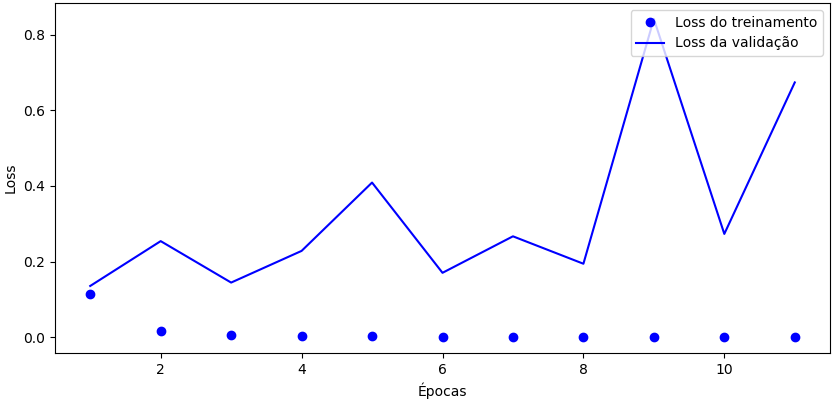
\includegraphics[width=0.45\textwidth]{imgs/lenet-a-loss}
	}
	\hfill
	\subfloat[Acurácia durante treinamento da melhor rede LeNet com a abordagem A.\label{subfig:lenet-a-acc}]{%
	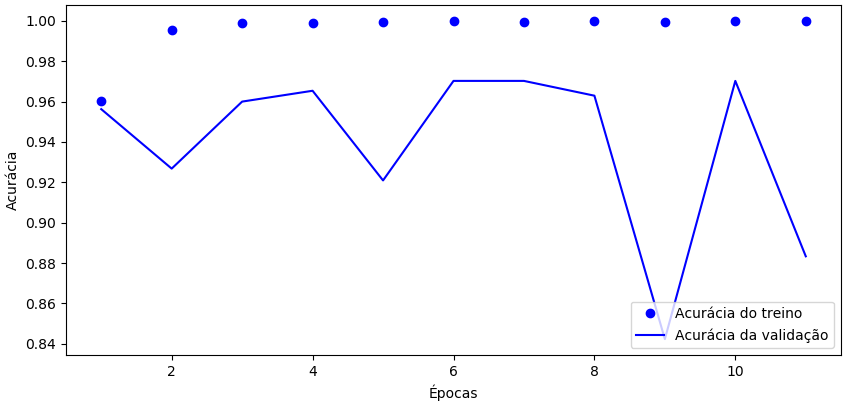
\includegraphics[width=0.45\textwidth]{imgs/lenet-a-acc}
	}
	\hfill
	\subfloat[\emph{Loss} durante treinamento da rede LeNet B.\label{subfig:lenet-b-loss}]{%
	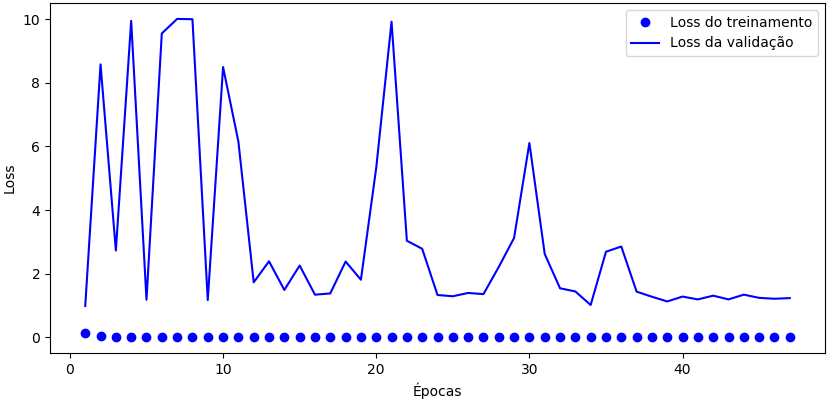
\includegraphics[width=0.45\textwidth]{imgs/lenet-b-loss}
	}
	\hfill
	\subfloat[Acurácia durante treinamento da rede LeNet B.\label{subfig:lenet-b-acc}]{%
	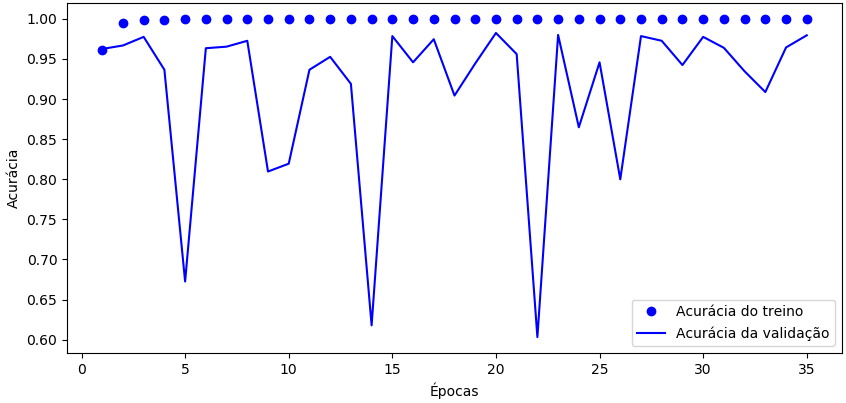
\includegraphics[width=0.45\textwidth]{imgs/lenet-b-acc}
	}
	\label{fig:treinamento-lenet}
\end{figure}

Examinando mais atentamente o desempenho destas redes no conjunto de testes, tem-se, então, as matrizes de confusão mostradas na Figura \ref{fig:matrizes-lenet}. Nestas matrizes, a soma das linhas representam a quantidade de assinaturas previstas para cada classe pelo modelo em questão, enquanto a soma das colunas denotam a quantidade de assinaturas existentes em cada classe.

\begin{figure}[h]
	\centering
	\caption{Matrizes de confusão dos melhores modelos obtidos com a arquitetura LeNet.}\label{fig:matrizes-lenet}
	\subfloat[Melhor LeNet com a abordagem A\label{subfig:matriz-lenet-a}]{%
	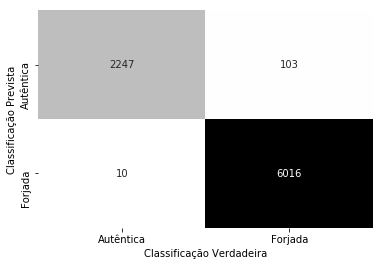
\includegraphics[width=0.47\textwidth]{imgs/matriz-lenet-a}
	}
	\hfill
	\subfloat[Melhor LeNet com a abordagem B\label{subfig:matriz-lenet-b}]{%
	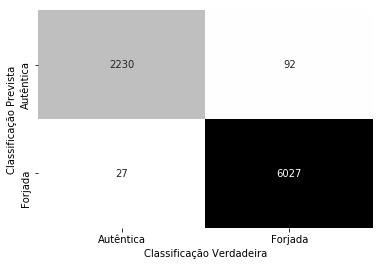
\includegraphics[width=0.47\textwidth]{imgs/matriz-lenet-b}
	}
\end{figure}

%%%% ARGUMENTAÇÃO

Para esta arquitetura, é possível visualizar que, dentre os dois modelos tidos como melhores, não há qualquer semelhança entre os hiperparâmetros encontrados. O número de épocas para aprendizado de características foi baixo para abordagem A, enquanto que, para a abordagem B, houve a necessidade de mais épocas de treinamento. Isso aconteceu, possivelmente, pela aparição de um mesmo autor em partições de dados diferentes na abordagem A.

A partir das matrizes de confusão, percebeu-se que o melhor modelo da abordagem A tendeu a verificar um baixo número de falsos negativos, ou seja, os exemplos autênticos foram suficientes para identificar assinaturas originais, indepentemente das variações cometidas por este autor. Por outro lado, para o modelo da abordagem B, verificou-se um número menor de falsos positivos, validando que, apesar da boa capacidade de certos forjadores \emph{over-the-shoulder} em realizar reproduções verossímeis, este modelo mostrou uma alta competência na detecção deste tipo de assinaturas. Não obstante, nota-se a diagonal principal de ambos os modelos bastante densa, sugerindo uma boa adequação para a tarefa considerada.
